% -*- TeX-master: "main"; fill-column: 72 -*-

\section{The Cell Behavior Ontology and the \token{cboTerm} attribute}
\label{sec:CBO}

It is difficult to determine the semantics of \Event constructs used to model intrinsic cellular behavior from SBML attributes alone. The \token{id} attribute on \Event objects allows for unique identification and cross-referencing while the \token{name} attribute allows the assignment of human readable labels to Events. Possible values for these attributes are unrestricted so that modelers can choose whichever fits their modeling framework and preference best. However, this means that without any additional human intervention, software tools are unable to discern the semantics of an extended \Event element modeling dynamic behavior. For instance, it would be inadvisable to interpret that an \Event is modeling the process of cellular death even if the \token{id} and \token{name} of such \Event have the \primtype{string} \val{Cell Death} as value. Additionally, as one may need to convert a dynamic \Event between different representations (e.g., Cellular Potts Model vs. Center-based off-lattice Model), there is a need to provide a standard, framework-independent, way of associating \Event components with given cellular processes.

A solution inspired by \sbmlthreecore is to associate model components with terms from carefully curated controlled vocabularies (CVs). This is the purpose of the \token{cboTerm} provided through the extended \SBase class in \sec{subsec:extSBase}. The \token{cboTerm} facilitates the annotation of \Event components, among others, with terms belonging to the Cell Behavior Ontology (CBO) \citep{Sluka2014}. In this section, we discuss \textbf{CBO}, its usage in SBML models via the \token{cboTerm} attribute and relevant modeling implications in the case of \Event objects.

\subsection{Cell Behavior Ontology (CBO)}
\label{subsec:bioCBO}

The development and use of bio-ontologies stems from the need to characterize and describe domains of biology in a standard way. The Cell Behavior Ontology (CBO) provides a carefully curated, controlled vocabulary that can be used to describe the behavior of a cell over time (dynamics) in a framework-independent manner, which enables the reliable exchange of biological descriptions. The Dynamic Structures SBML extension allows modelers to use available CBO identifiers to tag SBML components via its attribute \token{cboTerm} to make the underlying biology and spatiality of the cellular process being modeled more explicit. The relationship between a \token{cboTerm} term describing an SBML component and the CBO term being used is of the form "the component is-A X", where X is the CBO term. Though CBO support provides an important source of information to understand the meaning of extended \Event elements, software does not need to support CBO terms to be considered SBML compliant.

The presence of a \token{cboTerm} attribute in an extended \Event is understood to change the way the \Event is interpreted and simulated. Annotating SBML \Event elements with CBO terms adds necessary semantic information that may be used to convert such \Event from one framework to another when shared; it enables software tools to recognize precisely what cellular behavior this component is meant to model. For example, if the \token{cboTerm} has the value of \url{http://cbo.biocomplexity.indiana.edu/svn/cbo/trunk/CBO_1_0.owl#CellDeath} for a given \Event, regardless of the value that the \token{id} or \token{name} attributes are given or the modeling method used, the \Event labeled with this ontological term will be understood to model the dynamics of cellular death.

\subsection{Using CBO and cboTerm}
\label{subsec:CBOTerm&CBO}

The \token{cboTerm} attribute is always of \primtype{CBOTerm} data type, as defined in \sec{attr:cboTerm}. When present, the attribute's value must be the full identifier of a single term taken from the Cell Behavior Ontology. The term chosen should be the most precise one that best summarizes the agent or phenomenon represented by a given SBML component. The relationship indicated by the presence of a non-empty \token{cboTerm} attribute in an \Event, for instance, is of the form "the Event is-A X", where X is the CBO term. 

\subsubsection{Structure of the Cell Behavior Ontology}
\label{subsec:CBOstructure}

The purpose of CBO is to standardize the description of intrinsic physical and biological characteristics of cells and tissues, which provides a basis for describing the spatial and observable dynamic behavior of cells in SBML models. To achieve this, CBO is split into controlled vocabularies for \textbf{CBO\textunderscore Objects}, which describe the physical entities of a biological model and \textbf{CBO\textunderscore Processs}, which describe the processes that aforementioned objects participate in. \ref{fig:CBOHierarchy} illustrates the taxonomy of CBO at the highest level.

\begin{figure}[tbhp]
	\centering
	%\usepackage{graphicx}
	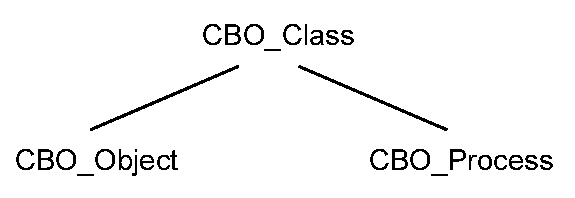
\includegraphics[width=0.25\textwidth]{images/CBO_Hierarchy.pdf}\\
	\caption{The controlled vocabularies that make up the main branches of CBO.} \label{fig:CBOHierarchy}
\end{figure}

As this SBML extension uses CBO as a reference ontology for the description of modeling elements inheriting from \SBase, the vocabulary supported in this extension is taken from both the \textbf{CBO\textunderscore Object} and \textbf{CBO\textunderscore Process} branches. Each of these  branches has a hierarchy of terms underneath them which may be represented by different SBML components. At this time, we can only begin to list some initial concepts and terms of CBO; what follows is not meant to be complete, comprehensive or even necessarily consistent with future versions of CBO. The website for CBO (\url{http://bioportal.bioontology.org/ontologies/CBO}) should be consulted for a current version of the ontology.

\subsubsection{CBO\textunderscore Object branch}
\label{subsubsec:CBOObjectBranch}

\begin{figure}[tbhp]
	\centering
	%\usepackage{graphicx}
	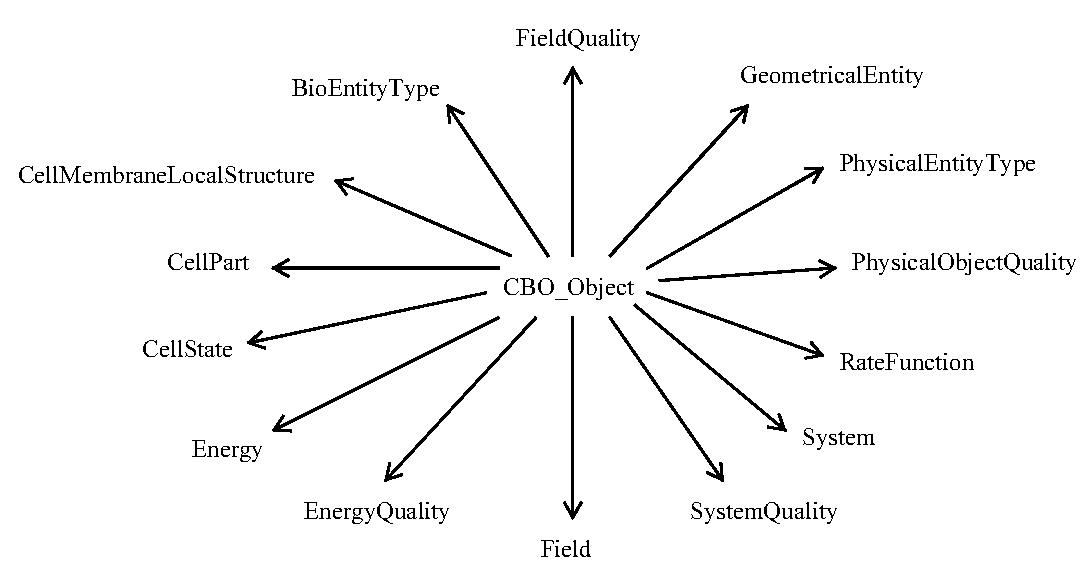
\includegraphics[width=0.60\textwidth]{images/CBO_ObjectBranch}\\
	\caption{The controlled vocabularies that make up the \textbf{CBO\textunderscore Object} branch.} \label{fig:CBOObjectBranch}
\end{figure}

\ref{fig:CBOObjectBranch} shows the structure of the \textbf{CBO\textunderscore Object} branch, which describes cell and non-cellular tissue components. As the CBO represents entities of a biological model as agents with the characteristics of physical objects, this branch includes terms to represent physical objects such as cells, membranes and cross-sections. Sub-branches such as the \textbf{BioEntityType}, \textbf{CellMembraneLocalStructure}, \textbf{CellPart} and \textbf{GeometricalEntity} each posses hierarchical groupings of the types of physical entities that can be represented in SBML by the \Compartment and \Species components. These include, but are not limited to cells, extracellular fluid/matrix, cellular structures such as filopodium in the case of motile cells and cellular regions such as the nucleus or cytoplasm.

The \textbf{CBO\textunderscore Object} hierarchy also contains terms that enable the quantitative description of these biological entities. Hierarchies of these terms include sub-branches such as \textbf{PhysicalObjectQuality} and \textbf{Energy}, which indicate object properties such as mass, age, electrical or energy functions for physical objects. This controlled vocabulary for quantitative parameters or functions is best mapped in SBML by the \Parameter and \FunctionDefinition objects. 

Also, defined under the \textbf{CBO\textunderscore Object} substructure are classes of ontological terms that represent concepts associated with the SBML \Parameter and \Model objects. The \textbf{System\textemdash model} and \textbf{SystemQuality\textemdash model} branches posses groupings for the description of model extents, computational platform and system boundaries.

\subsubsection{CBO\textunderscore Process branch}
\label{subsubsec:CBOProcessBranch}

\ref{fig:CBOProcessBranch} shows the structure of the \textbf{CBO\textunderscore Process} branch, which describes processes involving physical agents such as cells. This branch includes hierarchies such as \textbf{CellProcess}, \textbf{StructuralProcess}, \textbf{FundamentalPhysicalProcess} and \textbf{MoleculeProcess} that serve to describe existential processes of cells and molecules- i.e., dynamic behavior. Examples of supported processes are cell\textendash cell adhesion, cell division and cell death, as well as existential processes of other model components such as molecule transport, diffusion, creation and destruction. The aforementioned branches posses hierarchical groupings of the types that are traditionally represented in SBML through either the \Reaction, \Rule or \Event elements. 

\begin{figure}[tbhp]
	\centering
	%\usepackage{graphicx}
	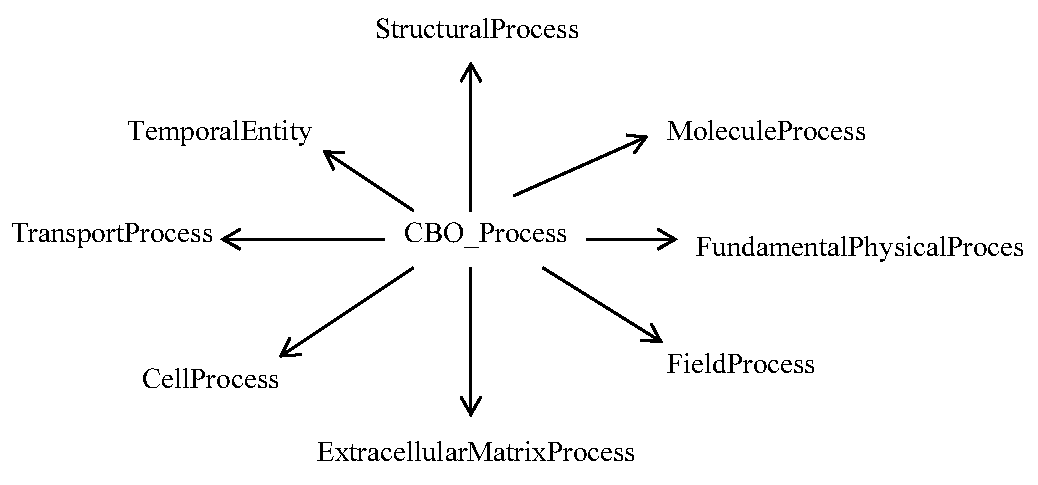
\includegraphics[width=0.60\textwidth]{images/CBO_ProcessBranch}\\
	\caption{The controlled vocabularies that make up the \textbf{CBO\textunderscore Process} branch.} \label{fig:CBOProcessBranch}
\end{figure}

\subsubsection{CBO and the \Event SBML component}
\label{subsubsec:supportedCBO}

One of the mechanisms the Dynamic Structures package uses to support the modeling of dynamic cellular behavior is the extension of the \SBase asbtract class to both annotate SBML components and impart specific simulation semantics to the \Event construct. Under this extension, \Event objects may carry a \token{cboTerm} attribute, whose value must be a full term identifier taken from the \textbf{CBO\textunderscore Process} vocabulary branch, which describes the behavior modeled by said \Event. Given substantial community input, the initial version of this package supports a handful of dynamic cellular behaviors. \ref{fig:allowedCBO} displays supported dynamic processes and their corresponding CBO terms. This table is preliminary and should not be taken as complete. It is merely intended to provide a formalism for the cross-platform interpretation and execution of CBO-annotated \Event constructs.

\begin{table}[h]
	\begin{tabular}{@{}ll@{}}
		\toprule
		\multicolumn{1}{c}{\textbf{Cell Behaviors}} & \multicolumn{1}{c}{\textbf{ CBO Terms}}                                   \\ \midrule
		Cell Division                              & http://cbo.biocomplexity.indiana.edu/svn/cbo/trunk/CBO\_1\_0.owl\#CellDivision        \\
		Cell Death                                 & http://cbo.biocomplexity.indiana.edu/svn/cbo/trunk/CBO\_1\_0.owl\#CellDeath           \\
		Cell Movement                       & 
		http://cbo.biocomplexity.indiana.edu/svn/cbo/trunk/CBO\_1\_0.owl\#Movement \\ \bottomrule
	\end{tabular}
		\caption{Subset of supported cellular behaviors and corresponding CBO terms} \label{fig:allowedCBO}
\end{table}

The following list contains a description of specific simulation semantics for each of the behaviors shown in \ref{fig:allowedCBO} when present in an \Event. A description of how other constructs are affected as a result of each behavior is also provided. \sbmlthreedynamic requires that sofware wishing to support dynamic cellular processes, understand the CBO vocabulary defined below: 


\begin{itemize}
	\item A \textbf{\textit{Cell Division}} term as value for the \token{cboTerm} attribute indicates that the \Event defines, by means of a \Trigger subobject, the mathematical conditions under which cellular division is to take place. When the \token{applyToAll} \Event attribute is set to \val{false}, the presence of this CBO term also dictates that model components whose \token{id} is referenced by an \Element in the \ListOfElements subobject have to be duplicated into a daughter cell. Quantities of the respective species and size of the compartments are set to half of the original in the case of symmetric cell division. When the value of \token{applyToAll} is \val{true}, all model elements are duplicated. 
	
	\item A CBO term for \textbf{\textit{Cell Death}} as value for a \token{cboTerm} attribute indicates that the \Event defines, by means of a \Trigger subobject, the mathematical conditions under which cell death is to take place. When the \token{applyToAll} \Event attribute is set to \val{false}, the presence of this CBO term also dictates that SBML model components whose \token{id} is referenced by an \Element in the \ListOfElements subobject have to be removed from the model. When the value of \token{applyToAll} is \val{true}, all model elements are removed. 	
	
	\item A CBO term for \textbf{\textit{Movement}} as value for a \token{cboTerm} attribute indicates that the \Event defines, by means of its \Trigger suboject, the mathematical conditions under which cell movement is to take place. When the \token{applyToAll} \Event attribute is set to \val{false}, the presence of this CBO term also dictates that SBML model \Compartments whose \token{id} is referenced by an \Element in the \ListOfElements subobject will have their position updated according to the force vector defined as a \SpatialComponent. When the value of \token{applyToAll} is \val{true}, the spatial location of all model \Compartments is also updated.

\end{itemize}

Although the use of CBO can be beneficial on elucidating the role of modeling elements, it is critical to keep in mind that the presence of a \token{cboTerm} value on an object does not change the fundamental mathematical meaning of the model. SBML models must be defined in a way, so that they stand on their own without depending on additional information added by CBO terms for a correct mathematical interpretation. In the case of labeled \Event elements, CBO term definitions will only imply alternative simulation semantics. Though tools not supporting these specific \Event semantics will not be able to reproduce dynamic behaviors as intended, they will be able to understand the meaning of said \Event. Allowing the use of \token{cboTerm} in \Event elements to alter the mathematical meaning of a model would allow too much leeway to slip inconsistent concepts into SBML objects, ultimately reducing model interoperability.

\subsubsection{Tradeoffs in using CBO terms}
\label{subsec:tradeoffCBO}

The presented CBO-based approach to annotating SBML \Event components with controlled terms has, just like the SBO-based approach presented in \sbmlthreecore, the following strengths:

\begin{enumerate}
	\item The syntax required is very straight-forward and requires a single \primtype{string} containing the \primtype{id} of a supported CBO term.
	\item Supported CBO terms cover a relevant portion of the cellular behaviors required by the community.
	\item It does not interfere with already-existing annotation schemes implemented by either Core and SBML extensions.
\end{enumerate}

The following list illustrates some of the weaknesses of the proposed approach:

\begin{enumerate}
	\item The Cell Behavior Ontology is a recent and evolving ontology. As such, it is susceptible to minor changes in its hierarchical taxonomy. These however, should not affect the \token{ids} of the terms themselves but rather the structure of the ontology itself.
\end{enumerate}

{\color{red} Harold: \notice Can we think of any other benefits or weaknesses?}

\subsubsection{Relationships to the SBML annotation element}
\label{subsubsec:CBO&Annot}

A common mechanism used to provide information regarding modeled dynamic cellular behaviors is the \token{sBase} \Annotation component. Annotations are commonly used by software tools, which generally have their own vocabulary for supporting similar cellular behaviors. However, the best-practice recommendation for interoperability is to use the \token{cboTerm} attribute in the \Event object rather than an \Annotation component. Software tools are encouraged to translate their tool-specific \Annotation schemes to the proposed \textbf{CBO-based} approach when writing SBML models that include dynamic cellular behaviors.
